\section{Action mécanique}
%
Un homme pousse un chariot, le chariot se met en mouvement. L'homme exerce une action mécanique,
c'est une action dite \textbf{\textit {de contact}} (il y a un contact entre l'acteur de l'action et le receveur), son effet est la mise en mouvement du chariot.

Une action mécanique est modélisée par une force. La force est un ensemble de caractéristique (intensité, direction, sens, point d'application), elle est représentée par un vecteur {\it partant} du point d'application.

\begin{center}
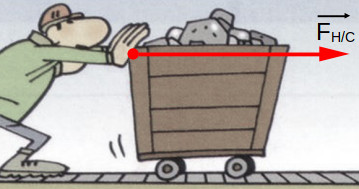
\includegraphics[scale=0.6]{./forces/chariotPousseForce}

\vspace{0.1cm}
$\overrightarrow{F_{H/C}}$ : Force exercée par l'Homme sur le Chariot.
\end{center}

Certaines actions mécaniques se produisent sans contact mécanique entre l'acteur et le receveur. Elles sont dites \textbf{\textit {à distance}}. Les paragraphes suivants donnent des exemples.

